\documentclass[12pt]{scrartcl}
\usepackage[ngerman]{babel}


\usepackage{amsmath, amssymb}

\usepackage{array}  % for the tables

\usepackage{nameref}  % for referencing with name

\usepackage{hyperref}  % for hyperlinks

\usepackage{mathrsfs}

\usepackage{graphicx}  % for the images

\usepackage{xcolor, colortbl}

\usepackage{gensymb} % for \degree

\usepackage{pgfplots}

\usepackage{tabto}

\newcolumntype{P}[1]{>{\centering\arraybackslash}p{#1}}

\usetikzlibrary{arrows}

% \usepgfplotslibrary{external}

% \tikzexternalize

\definecolor{Gray}{gray}{0.85}

\setlength{\parindent}{0cm}

% hyperlinks
\hypersetup{
    colorlinks,
    citecolor=black,
    filecolor=black,
    linkcolor=black,
    urlcolor=black
}

\bibliographystyle{IEEetran}




\author{David Jäggli}

\title{Diskrete Mathematik}



% ---------- Begin Main Document ----------- %



\begin{document}

\maketitle

\tableofcontents

\newpage
\section{Allg}

\subsection{Grundlagen der Logik und Beweise}

\begin{itemize}
    \item Die Regeln der Logik geben mathematischen Aussagen eine präzise Bedeutung.
    \item Konstruktion korrekter mathematischer Argumente
\end{itemize}

\subsection{Aussagen (Propositionen)}
\textbf{Propositionen:}
\begin{itemize}
    \item Bern ist die Bundesstadt
    \item 1 + 1 = 2
    \item Goldbachsche Vermutung: sie ist entweder wahr oder falsch, man weis es noch nicht
\end{itemize}

\textbf{Keine Propositionen:}
\begin{itemize}
    \item Wie spät ist es?
    \item x + 1 = 2
    \item Dieser Satz ist falsch.
\end{itemize}

Begründung: Es handelt sich hier nicht um Aussagen, die entweder wahr oder falsch sind.
Eine Aussage ist wahrheitsdefiniert. In einer Aussage darf nicht offen sein ob die Aussage wahr oder 
falsch sein kann. Sie darf sich auch nicht selbst widersprechen.

% ------------------------------------------------------
\section{Operatoren}

\begin{itemize}
    \item Negotiationsoperator: $\lnot$
    \item Konjunktion $\land$
    \item Disjunktion $\lor$
    \item Implikation $\rightarrow$
    \item Bikonditional $\leftrightarrow$
\end{itemize}



\subsection{Diskunktion}
$p \lor q$\\
Wenn p oder q wahr ist, ist die Aussage wahr (logic OR).


\renewcommand{\arraystretch}{1.5}
\begin{tabular}{ | m{3em} | m{3em} | m{3em} | }
    \hline
    p & q & $p \lor q$\\ 
    \hline
    w & w & w\\ 
    \hline
    w & f & w\\ 
    \hline
    f & w & w\\ 
    \hline
    f & f & f\\ 
    \hline
\end{tabular}


\subsection{Implikation}
$p \rightarrow q$\\
Wenn p dann q


\renewcommand{\arraystretch}{1.5}
\begin{tabular}{ | m{3em} | m{3em} | m{3em} | }
    \hline
    p & q & $p \rightarrow q$\\ 
    \hline
    w & w & w\\ 
    \hline
    w & f & f\\ 
    \hline
    f & w & w\\ 
    \hline
    f & f & w\\ 
    \hline
\end{tabular}


\subsection{Bikonditional}
$p \leftrightarrow q$\\
Wenn beide den gleichen Wahrheitswert haben ist die Aussage wahr.\\
\textbf{Wahrheitstabelle:}\\

\renewcommand{\arraystretch}{1.5}
\begin{tabular}{ | m{3em} | m{3em} | m{3em} | }
    \hline
    p & q & \(p \leftrightarrow q\)\\ 
    \hline
    w & w & w\\ 
    \hline
    w & f & f\\ 
    \hline
    f & w & f\\ 
    \hline
    f & f & w\\ 
    \hline
\end{tabular}

\subsection{Prioritäten}
\renewcommand{\arraystretch}{1.5}
\begin{tabular}{ | m{4em} | m{4em} | }
    \hline
    Operator & Priorität\\ 
    \hline
    $\lnot$ & 1\\ 
    \hline
    $\land$ & 2\\ 
    \hline
    $\lor$ & 2\\ 
    \hline
    $\rightarrow$ & 3\\ 
    \hline
    $\leftrightarrow$ & 3\\ 
    \hline
\end{tabular}


\section{Aussagen}

\subsection{Tautologie und Wiederspruch}
Tautologie ist eine Aussage, welche immer wahr ist.\\
Ein Wiederspruch ist eine Aussage, welche immer falsch ist.

\subsection{Logische Äquivalenzen}
Die Aussage p und q heissen logisch äquivalent, falls \(p \leftrightarrow q\) eine Tautologie ist. 
Man schreibt dann \(p \Leftrightarrow q\) oder
\(p \equiv q\) bzw. $p \sim q$

\subsection{Logische Äquivalenzregeln}
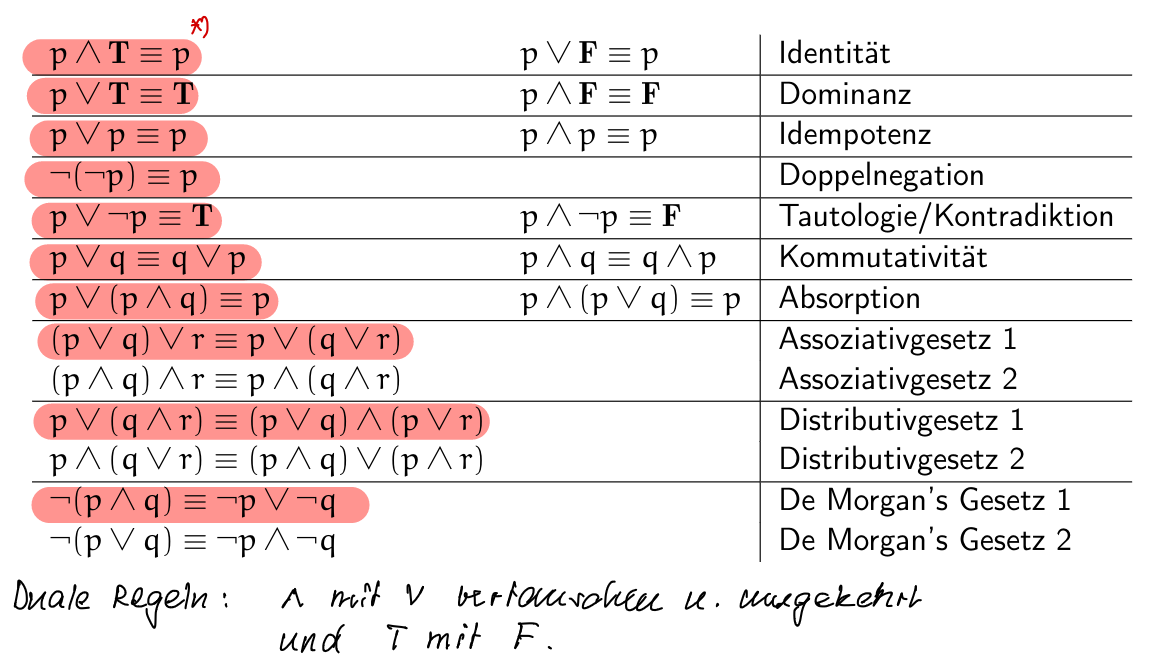
\includegraphics[width=14cm]{img/logic_equivalence_rules.png}

Weiterführend:\\
$p \rightarrow q \equiv \lnot p \lor q$


\newpage
\textbf{Beispiel angewandte logische Äquivalenzregeln}\\
Beispiel 1:\\
$\left(p \lor \lnot(q \land p)\right) \land \left(r \lor (s \lor r)\right)$\\
$\equiv (p \lor \lnot q \lor \lnot p) \land (r \lor r \lor s)$\\
$\equiv (T \lor \lnot q) \land (r \lor s)$\\
$\equiv T \land (r \lor s)$\\
$\equiv r \lor s$
 \\
 \\
 \\

Beispiel 2:\\
$(a \rightarrow (b \rightarrow c)) \rightarrow ((a \rightarrow b)\rightarrow (a \rightarrow c))$\\
$\equiv (a \rightarrow (\lnot b \lor c)) \rightarrow ((\lnot a \lor b) \rightarrow (\lnot a \lor c))$\\
$\equiv (\lnot a \lor (\lnot b \lor c)) \rightarrow (\lnot(\lnot a \lor b) \lor (\lnot a \lor c))$\\
$\equiv (\lnot a \lor \lnot b \lor c) \rightarrow ((a \land \lnot b) \lor \lnot a \lor c)$\\
$\equiv (\lnot a \lor \lnot b \lor c) \rightarrow ((a \lor \lnot a) \land (\lnot b \lor \lnot a) \lor c)$\\
$\equiv (\lnot a \lor \lnot b \lor c) \rightarrow (\lnot b \lor \lnot a \lor c)$\\
$\equiv$ X $\rightarrow$ X\\
$\equiv \lnot$X $\lor$ X\\
$\equiv$ T\\

\section{Quantoren}
Wird ein Quantor auf die Variable x angewandt, dann nennt man diese Variable \textit{gebunden}, ansonsten \textit{frei}.
\subsection{Prädikate}
Ein Prädikat ist ein Wortkonstrukt, welches mindestens eine Variable enthält.\\
$P(x) =$ ''$x > 3$''\\
Die Aussage $P(4) = 4 > 3$ ist wahr, während $P(2) = 2 > 3$ falsch ist.

\subsection{Allquantor}
Ist $P(x)$ wahr für alle x aus einer bestimmten Universalmenge, dann schreibt man $\forall x P(x)$.
Gelesen wird dies, "für alle $x$ gilt $P(x)$".\\
Falls es nur auf eine Bestimmte Zahlenmenge zutrifft (z.B. $\mathbb{Z}$) dann schreibt man:\\
$\forall x \in \mathbb{Z}$ ist wahr.

\subsection{Existenzquantor}
Ist $P(x)$ wahr für mindestens ein $x$ aus einer bestimmten Universalmenge, dann schreibt man $\exists x P(x)$
und liest: "es existiert ein $x$ für welches $P(x)$ wahr ist".


\subsection{Verschachtelte Quantoren}
Die Reihenfolge der Quantoren ist wesentlich; ausser alle Quantoren sind vom gleichen Typ (also Allquantoren oder Existenzquantoren)!


\newpage
\section{Beweise}
\begin{itemize}
    \item Ein Satz (Theorem) ist eine Aussage, von der man zeigen kann, dass sie wahr ist.
    \item Um zu zeigen, dass ein Satz wahr ist, verwendet man eine Abfolge (Sequenz) von Aussagen, die zusammen ein Argument, genannt Beweis ergeben.
    \item Aussagen können Axiome oder Postulate enthalten (grundlegende Annahmen der mathematischen Strukturen).
    \item Durch logisches (also gewissen Regeln gehorchendes) schliessen werden Folgerungen gemacht, die zusammen den Beweis ergeben.
    \item Ein Lemma ist ein einfacher Satz, der in Beweisen von komplizierteren Sätzen verwendet wird.
    \item Ein Korollar ist eine einfache Folgerung eines Satzes.
\end{itemize}


% ----------- Mengen ----------- %

\newpage
\section{Mengen}

Eine Menge ist eine ungeordnete Zusammenfassung wohldefinierter, unterscheidbarer
Objekte, genannt \textit{Elemente}, zu einem Ganzen. Für irgendein Objekt $x$ 
gilt dann bezüglich der Menge $A$ entweder $x \in A$ oder dann $x \notin A$.

\textbf{Beispiel:}\\
Endliche Mengen lassen sich durch Aufschreiben der in ihnen enthaltenen Elemente beschreiben.
z.B. die Menge aller natürlichen Zahlen kleiner als 101:\\
$A = {0, 1, 2, ..., 99, 100}$ (aufzählend notiert)\\
$99 \in A$ aber $101 \notin A$ (beschreibend notiert)\\

andere Schreibweisen sind: \\

$A = {n \in \mathbb{N} | n < 101} = {n \in \mathbb{N} : n <= 100} = {n|n \in \mathbb{N} \land n <= 100}$\\

\subsection{Gleichheit, elementare Mengen}
Zwei Mengen $A$ und $B$ sind \textbf{gleich} ($A = B$), falls sie dieselben Elemente enthalten.
$(A \subset B) \land (B \subset A)$\\

\textbf{Einige bekannte Mengen:}\\
$\mathbb{N}$ - \quad Menge der natürlichen Zahlen $(\mathbb{N}^* = \mathbb{N} \setminus \{0\})$\\
$\mathbb{Z}$ - \quad Menge der ganzen Zahlen\\
$\mathbb{Z}^+$ - \quad Menge der positiven ganzen Zahlen\\
$\mathbb{Q}$ - \quad Menge der Brüche\\
$\mathbb{R}$ - \quad Menge der reellen Zahlen\\
$\mathbb{C}$ - \quad Menge der komplexen Zahlen\\

\subsection{Spezielle Mengen}
\textbf{Teilmenge:} $A$ ist Teilmenge von $B$, geschrieben $A \subset B$, genau dann, wenn
$\forall x (x \in A \rightarrow x \in B)$: es gilt $A \subset A$!\\

\textbf{Leere Menge:} Für jede Menge $A$ gilt: $\emptyset \subset A$.\\

\textbf{Kardinalität:} Ist $S$ eine endliche Menge, dann bezeichnet $|S|$ die Kardinalität. Die
Kardinalität ist die Anzahl Elemente von $S$.\\

\textbf{Potenzmenge}: Die Potenzmenge $P(S)$ oder $2^S$ der Menge $S$ besteht aus der Menge aller
Teilmengen $A \subset S$.\\

\textbf{Beispiel:}\\
Bestimmen Sie die Potenzmenge von $S= \{1,2\}$\\
$S = \{1,2\}$\\
\quad $P(S) = 2^S = \{\emptyset, \{1\}, \{2\}, \{1, 2\}\}$\\
Es gilt allgemein $|2^S| = 2^{|S|}$


\subsection{Das Kreuzprodukt zweier Mengen / kartesisches Produkt}
$ A \times B = \{(a, b)|a \in A \land b \in B\}$\\
Reihenfolge ist entscheidend, $A \times B \neq B \times A$\\
$|A \times B| = |A| \cdot |B|$\\

\textbf{Beispiel:}
$A \times B = \{(1,a), (2,a), (3,a), (1,b), (2,b), (3, b)\}$


\subsection{Mengenoperationen}
\subsubsection{Komplement}
Ist $A$ eine Teilmenge der Menge $M$, so bezeichnet\\

$A^c = \overline{A} =  \{m \in M | m \notin A\}$\\

das Komplement von $A$ bezüglich $M$.

\subsubsection{Durchschnitt}
Sind $A$ und $B$ Teilmengen einer Menge $M$, so bezeichnet\\

$A \cap B = \{m \in M | m \in A \land m \in B\}$\\

den  Durchschnitt von $A$ und $B$.


\subsubsection{Vereinigung}
Sind $A$ und $B$ Teilmengen einer Menge $M$, so bezeichnet\\

$A \cup B = \{m \in M | m \in A \lor m \in B\}$\\

die Vereinigung von $A$ und $B$.


\newpage
\subsubsection{Differenz}
Sind $A$ und $B$ Teilmengen einer Menge $M$, so bezeichnet \\

$B \setminus A = \{m \in M | m \in B \land m \notin A\}$\\

die Differenz


\subsection{Set Operatoren}
\renewcommand{\arraystretch}{1.5}
\begin{tabular}{ | m{7em} | m{7em} | }
    \hline
    Allg. Operator & Set Operator \\ 
    \hline
    $p \lor q$ & $A \cup B$ \\ 
    \hline
    $p \land q$ & $A \cap B$ \\ 
    \hline
    $\lnot p$ & $\overline{A} $ \\ 
    \hline
\end{tabular}

\subsubsection{Rechenregeln}
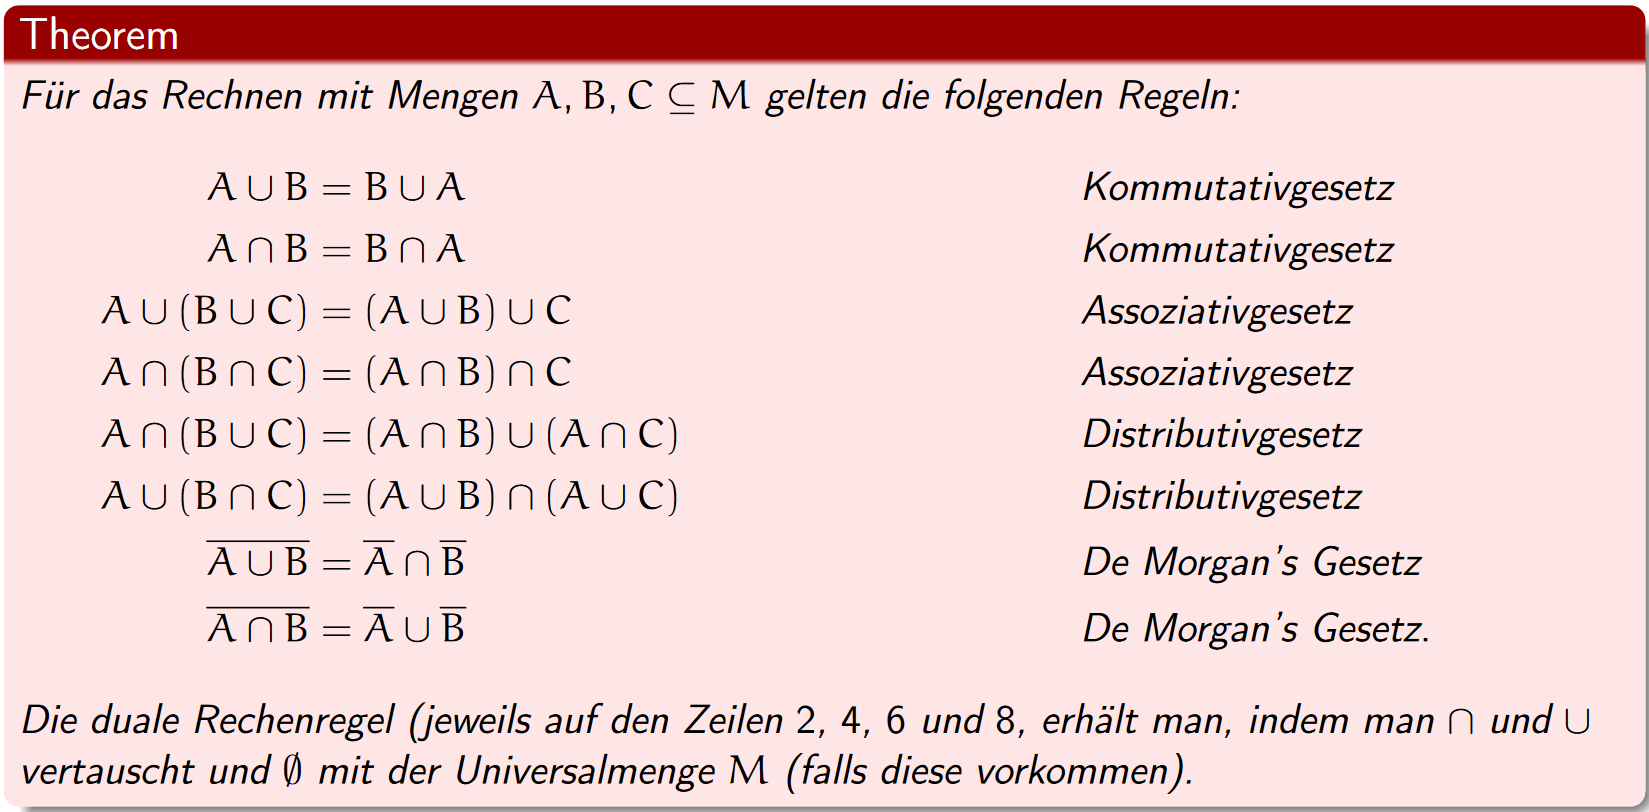
\includegraphics[width=15cm]{img/Rechenregeln_mit_mengen.png}

\subsubsection{Mengen Identitäten}
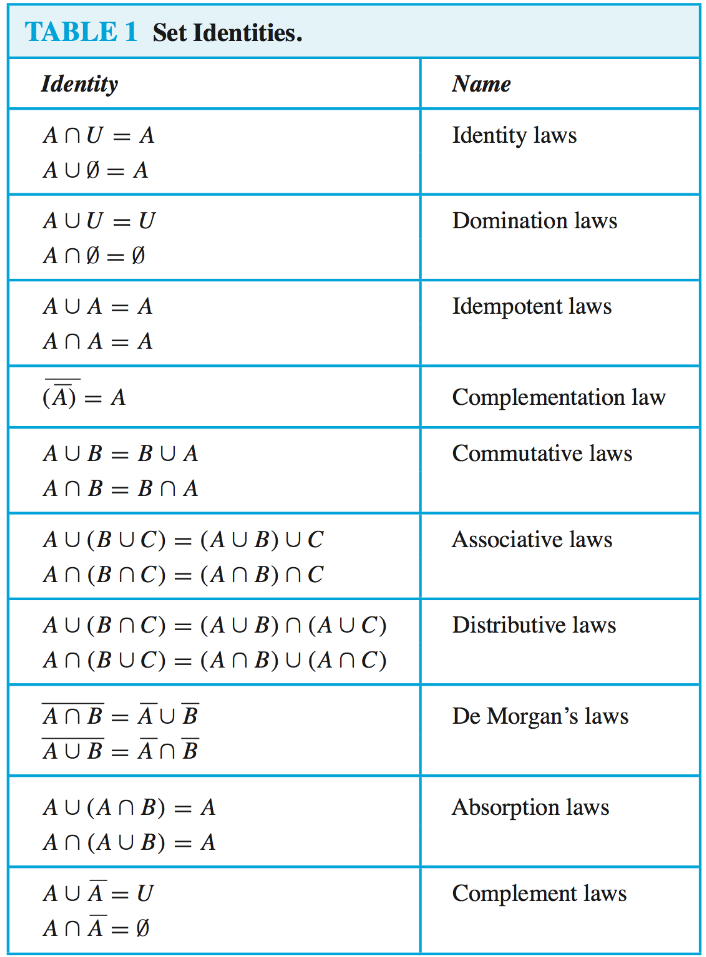
\includegraphics[width=15cm]{img/set_identities.png }




\section{Funktionen}
Wird jedem Element $x$ einer Menge $X$ genau ein Element $y$ einer Menge
$Y$ zugeordnet, so heisst die Zuordnung \textbf{Funktion}.


\subsection{Die ceiling- und floorfunction}
$\lceil \cdot \rceil$ :  $\mathbb{R} \rightarrow \mathbb{Z}$, $x \mapsto \lceil x \rceil =$ min$\{n \in \mathbb{Z} | x \leq n\}$\\
$\lfloor \cdot \rfloor$ :  $\mathbb{R} \rightarrow \mathbb{Z}$, $x \mapsto \lfloor x \rfloor =$ max$\{n \in \mathbb{Z} | n \leq x\}$\\


\subsection{Injektive Funktionen}
Eine Funktion heisst injektiv, wenn jedes $x$ auf eine eigenes $y$ zeigt.

\subsection{Surjektive Funktionen}
Eine Funktion heisst surjektiv, falls für jedes Element $y$ ein Element $x$ existiert, so dass $f(x) = y$ gilt.

\subsection{Bijektive Funktionen}
Eine Funktion heisst bijektiv, falls sie injektiv und surjektiv ist. Das bedeutet, dass jedes Element $y$ genau
ein zugehöriges Element $x$ hat.\\

Bijektive Funktionen sind umkehrbar. Man muss einfach die Pfeile umkehren und damit entsteht
aus $f$ die Umkehrfunktion $f^{-1}$.


\subsection{Zusammengesetzte Funktionen}
Gegeben seien zwei Funktionen, so dass der Wertebereich von $g$ im Definitionsbereich von $f$ enthalten ist.
Dann kann man die so genannte \textbf{zusammengesetzte Funktion} oder \textbf{Komposition} von $f$
und $g$ bilden:\\
$F = f \circ g$ : $X \longmapsto Y$, $x \longmapsto f(g(x))$


\subsection{Die Caesar-Chiffre}
\begin{enumerate}
    \item \textbf{Kodierung:} Buchstaben auf Zahlen abbilden\\
    K:\{$a$,$b$,$c$,...,$z$\} $\mapsto$ \{0,1,2,...,25\}, wobei $a \mapsto 0$,$b \mapsto 1$,$c \mapsto 2$,$z \mapsto 25$
    \item \textbf{Verschlüsseln:} die eigentliche Caesar-Verschlüsselung\\
    V:\{0,1,2,...,25\} $\mapsto$ \{0,1,2,...,25\}, $m \mapsto c := (m + 3)$ mod 26.
    \item \textbf{Dekodierung:} Zahlen auf Buchstaben abbilden\\
    D:\{0,1,2,...,25\} $\mapsto$ \{0,1,2,...,25\}, wobei $0 \mapsto a$,$1 \mapsto b$,$2 \mapsto c$,$25 \mapsto z$
\end{enumerate}


\subsection{Umkehrfunktionen}
Wenn man die Umkehrfunktion auf das Ergebnis der Ursprungsfunktion mit einem $x$-Wert anwendet
erhält man wieder $x$. Heisst:\\
$f^{-1}(f(x)) = x$


\newpage
\section{Folgen}
\subsection{Definition}
Eine \textbf{Folge} ist eine Abbildung von $\mathbb{N}$ (oder auch $\mathbb{N}^* = \mathbb{N} \setminus \{0\}$) in eine Menga $A$:\\
$\{\cdot\}$:$\mathbb{N} \mapsto A$, $n \mapsto a_n$\\
Man nennt $a_n$ das Glied der Folge mit der Nummer $n$. Die Folge wird auch mit \{$a_n$\} oder ($a_n$) bezeichnet.\\

\textbf{Example:}\\
Man schreibe die ersten sechs Glieder der Folge auf, deren k. Glied gegeben ist durch $a_k = \frac{1}{k}$. \\

$a_k = \left(1,  \dfrac{1}{2}, \dfrac{1}{3}, \dfrac{1}{4}, \dfrac{1}{5}\dots\right)$


\subsection{Die geometrische Folge}
Bei einer geometrischen Folge ist der Quotient zweier aufeinander folgender Glieder immer
gleich, nämlich q. Das bedeutet, dass $\frac{a_{k+1}}{a_k}$ immer gleich ist.


\subsection{Summen}
Dank Summenzeichen lassen sich Summen einfacher schreiben:
\[\sum_{j=m}^{n} a_j = a_m + a_{m+1} + a_{m+2} + \dots + a_n\]

\[\sum_{j=m}^{n} a_j = \sum_{i=0}^{n-m} a_{m+i} = \sum_{k=1}^{n-m+1} a_{m+k-1}\]


Addiert man die Glieder einer arithmetischen Folge ($a_k$), entsteht die \textbf{arithmetische Reihe:}

\[\sum_{k=0}^{n-1} a_k = n \frac{a_0 + a_{n-1}}{2}\]


\newpage
\textbf{Nützliche Summenformeln:}

\renewcommand{\arraystretch}{2.5}
\begin{center}
    \begin{tabular}{  m{10em} | P{10em} }
        \hline
        Summe & geschlossene Form \\
        \hline
        $\sum_{k=1}^{n} k$                          & $\dfrac{n(n + 1)}{2}$         \\ 
        $\sum_{k=1}^{n} k^2$                        & $\dfrac{n(n + 1)(2n + 1)}{6}$ \\ 
        $\sum_{k=1}^{n} k^3$                        & $\dfrac{n^2(n + 1)^2}{4}$     \\ 
        $\sum_{k=0}^{\infty} x^k$, $|x| < 1$        & $\dfrac{1}{1 - x}$            \\ 
        $\sum_{k=1}^{\infty} kx^{k-1}$, $|x| < 1$   & $\dfrac{1}{(1-x)^2}$          \\ 
        \hline
    \end{tabular}
\end{center}


\subsection{Produkte}
Dank dem Produktzeichen lassen sich Produkte einfacher schreiben:\\


\[a_m \cdot a_{m+1} \cdot a_{m+2} \dots a_n = \prod_{j=m}^{n} a_j \quad\quad n \geqslant m\]

Die Fakultät lässt sich mithilfe des Produktzeichens wie folgt schreiben:\\
\[n! = 
\begin{cases}
    1 & n=0 \\
    n(n - 1)(n - 2) \dots 2 \cdot 1 = \prod_{k=1}^{n}k & n > 0
\end{cases}\]


% tabular example 3 columns
% \renewcommand{\arraystretch}{1.5}
% \begin{center}
%     \begin{tabular}{ | m{12em} | m{12em} | m{12em} | }
%         \hline
%         1 & 2 & 3\\ 
%         \hline
%         1 & 2 & 3\\ 
%         \hline
%         1 & 2 & 3\\ 
%         \hline
%     \end{tabular}
% \end{center}


% tabular example 2 columns
% \renewcommand{\arraystretch}{1.5}
% \begin{center}
%     \begin{tabular}{ | m{17em} | m{17em} | }
%         \hline
%         1 & 2\\ 
%         \hline
%         1 & 2\\ 
%         \hline
%         1 & 2\\ 
%         \hline
%     \end{tabular}
% \end{center}


% \begin{tikzpicture}[line cap=round,line join=round,>=triangle 45,x=0.5cm,y=0.25cm]
%     \begin{axis}[
%     x=0.75cm,y=0.5cm, % size of the grid
%     axis lines=middle,
%     ymajorgrids=true,
%     xmajorgrids=true,
%     xmin=-10,
%     xmax=10,
%     ymin=-10,
%     ymax=10,
%     xtick={-11,-10,...,10},
%     ytick={-10,-9,...,9},]
%     \draw[line width=2pt,color=blue] (-10,-5) -- (-2,-1);
%     \begin{scriptsize}
%         \draw[color=blue] (-9.866,-4.728) node {$g$};
%         \draw[color=blue] (-1.906,7.172) node {$f$};
%         \draw[color=blue] (3.134,5.232) node {$h$};
%     \end{scriptsize}
% \end{axis}
% \end{tikzpicture}




% \bibliography{quantum_ready}

\end{document}